\documentclass[11pt,twocolumn,twoside]{opticajnl}
%% Please use 11pt if submitting to AOP
% \documentclass[11pt,twocolumn,twoside]{opticajnl}

\journal{pr} % Choose journal (ao,jocn,josaa,josab,ol,optica,pr)

%See template introduciton for guidance on setting shortarticle option
\setboolean{shortarticle}{True}
% true = letter/tutorial
% false = research/review article
% (depending on journal)
\usepackage{lineno}
\usepackage[utf8]{inputenc}
\spanishdecimal{.}
\usepackage{amsmath}
\usepackage{caption}
\usepackage{subcaption}
\usepackage[spanish]{babel}
\usepackage{hyperref}
\usepackage{listings}
\usepackage{multicol}
%\linenumbers

% Configura el formato del título del listado
\renewcommand\lstlistingname{Código}
\renewcommand\lstlistlistingname{Códigos}
\title{

\vspace{0.5cm} 

Trabajo práctico 2: Estadística de trenes de spikes}

\author[1]{\huge{Ignacio Lembo Ferrari}}
\affil[1]{\large{ignaciolembo@ib.edu.ar} 

\vspace{0.3cm}

\large{28 de septiembre de 2023.}

\vspace{0.5cm}
}

%\begin{abstract}
%\textbf{hola}
%\end{abstract}

\begin{document}

\maketitle

En este trabajo se estudiaron los datos experimentales medidos con electrodos intracelulares por Ariel Rokem en un receptor acústico de un saltamontes. El experimento realizado consistió en someter al animal a un estímulo acústico mientras se medía la actividad neuronal en ventanas de $0.1$ ms durante un tiempo total de $1000$ ms. Se realizaron 128 realizaciones del experimento.

Para el análisis de los datos y la obtención de los gráficos se desarrolló un programa en Python (ver apéndice \ref{codigo})

\section{Distribución de intervalos ISI de la neurona \label{sec:ISI}}

\vspace{0.3cm}

En primer lugar, se muestra en la Fig. \ref{fig:señal} la envolvente de la onda sonora que se le presentaba al saltamontes en cada realización del experimento. En la Fig. \ref{fig:realizaciones} se muestra un diagrama con las 128 realizaciones del experimento en función del tiempo, indicando con un punto si se produjo un spike en un dado tiempo para una dada realización. Se observan franjas donde la cantidad de spikes disminuye y franjas donde aumenta.

\begin{figure}[ht]
    \centering
         \begin{subfigure}[b]{\linewidth}
            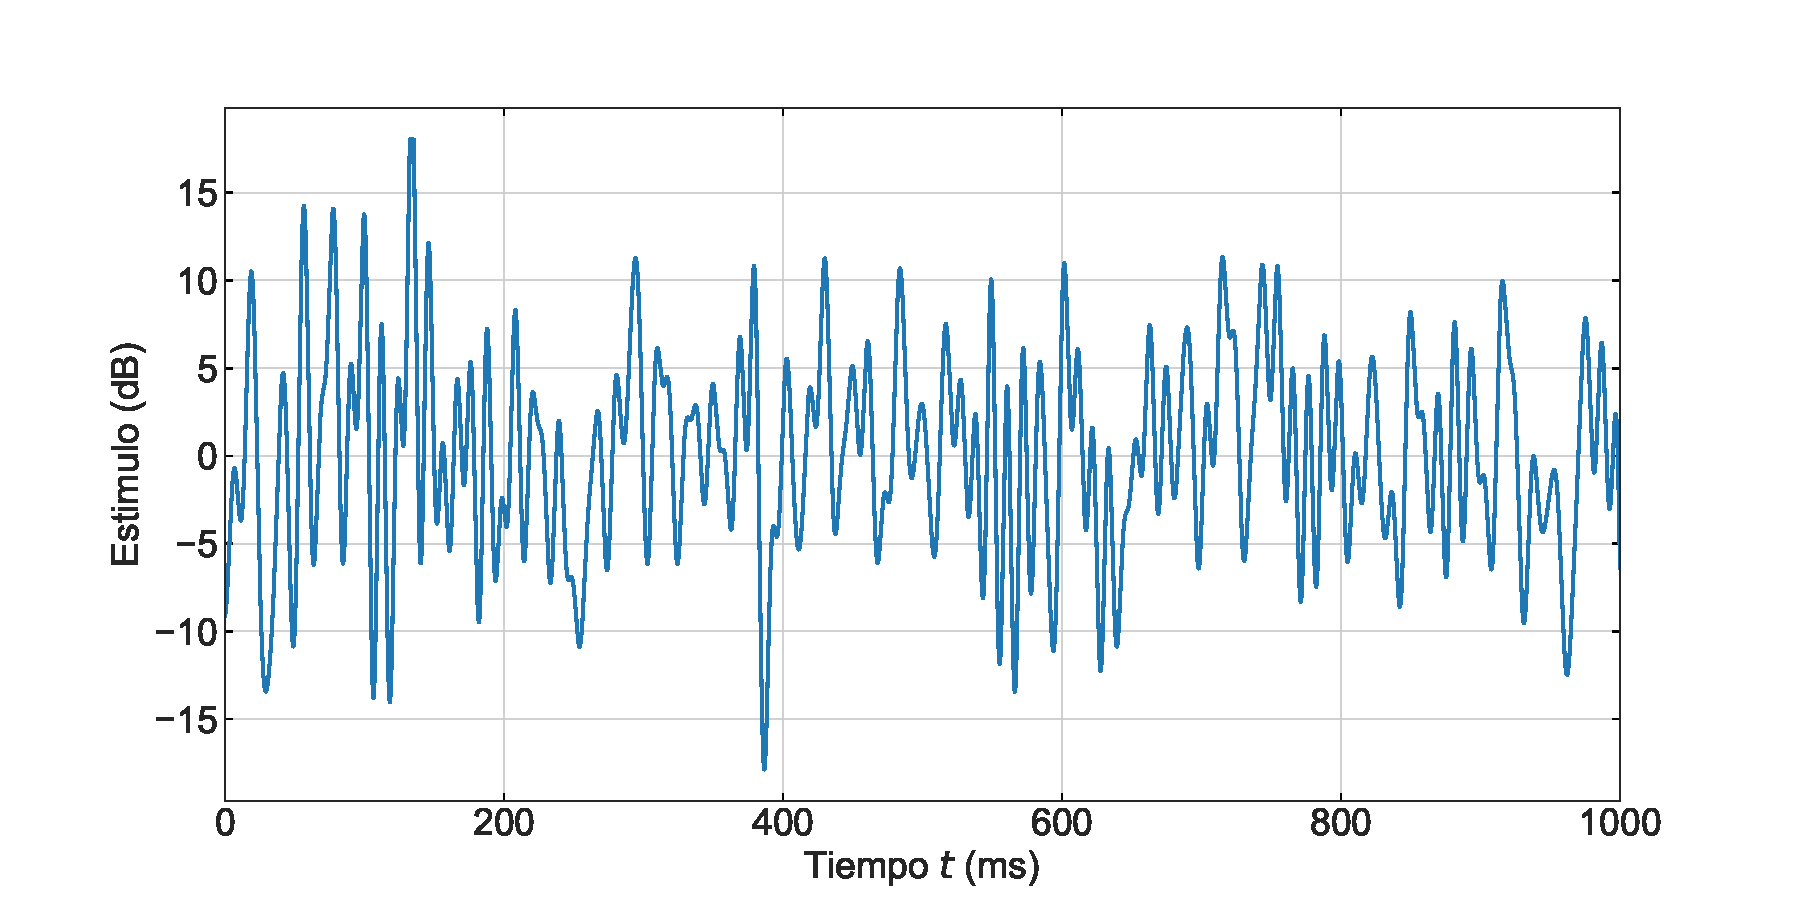
\includegraphics[width=\textwidth]{Figuras/estimulo_vs_t.pdf}
         \end{subfigure}
    \caption{Envolvente del estímulo utilizado en el saltamontes en función del tiempo} 
    \label{fig:señal}
\end{figure}
\begin{figure}[ht]
    \centering
         \begin{subfigure}[b]{\linewidth}
            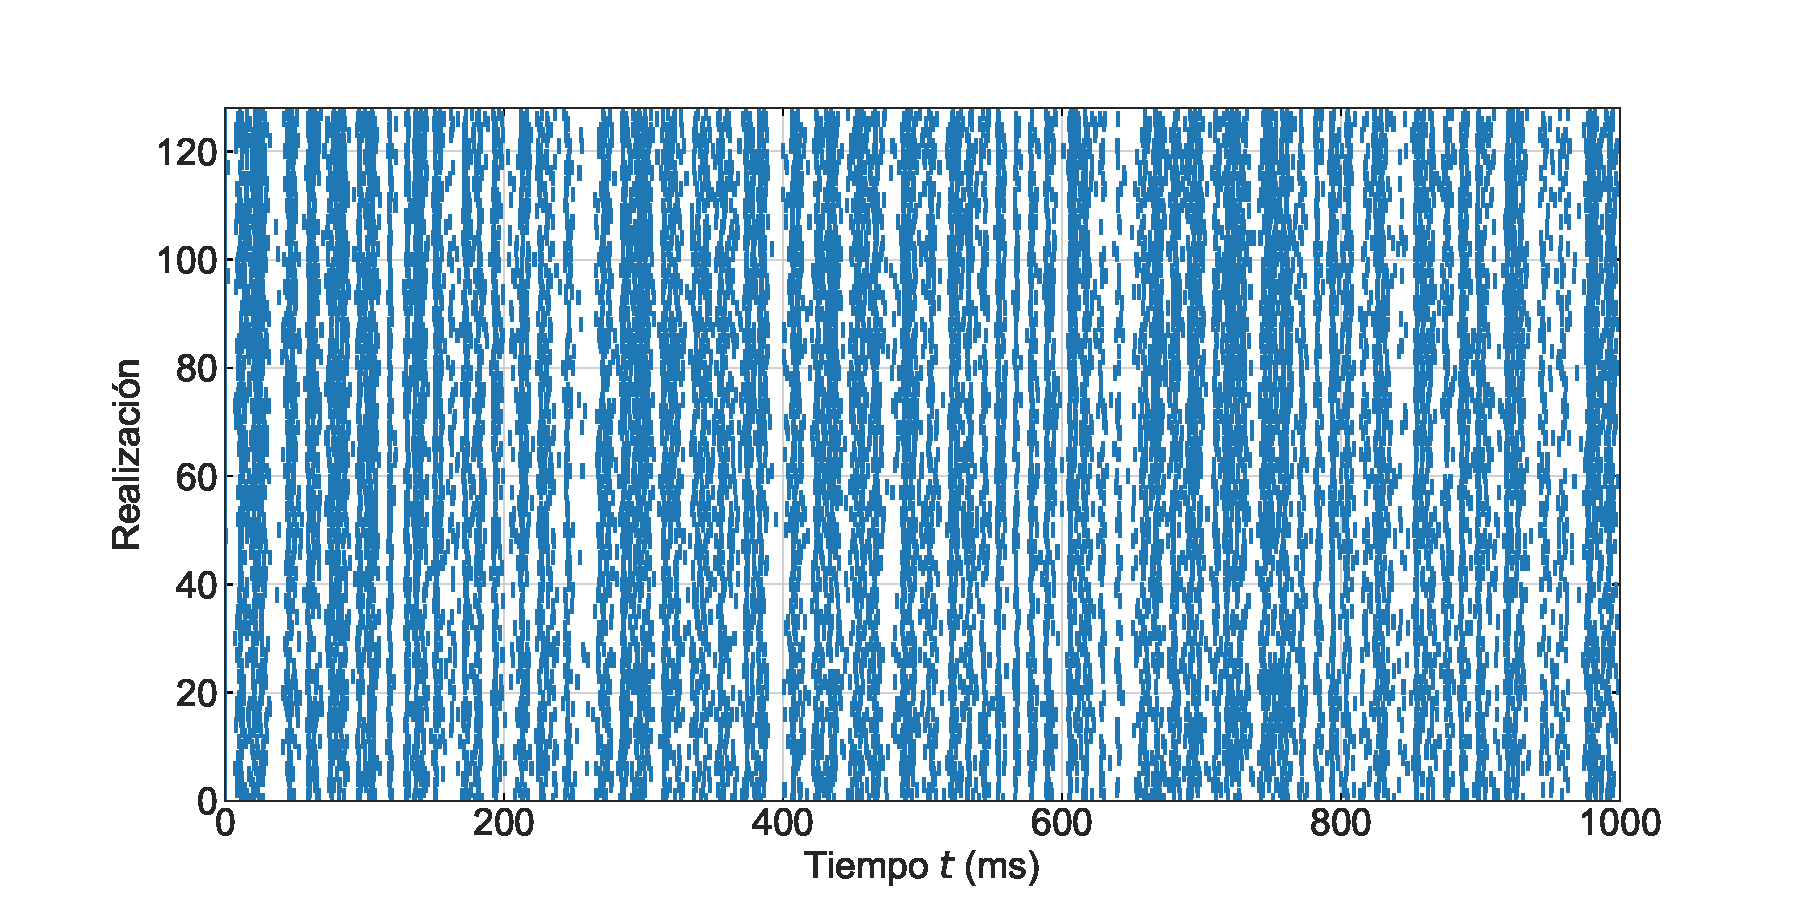
\includegraphics[width=\textwidth]{Figuras/reailzaciones_vs_t.pdf}
         \end{subfigure}
    \caption{Diagrama de spikes para cada realización. Cada fila representa uno de los 128 experimentos y cada punto un spike. El tiempo total de cada experimento fue de $1000$ ms, con ventanas de $0.1$ ms.} 
    \label{fig:realizaciones}
\end{figure}

Se realizó un histograma de la distribución de los intervalos de tiempo
entre disparos (inter-spike interval, ISI) para todos las realizaciones del experimento. El resultado se muestra en la Fig. \ref{fig:histISI}. Se observa que luego de un spike la neurona no vuelve a disparar durante un tiempo del orden de $5$ ms aproximadamente.
\begin{figure}[H]
    \centering
         \begin{subfigure}[H]{\linewidth}
            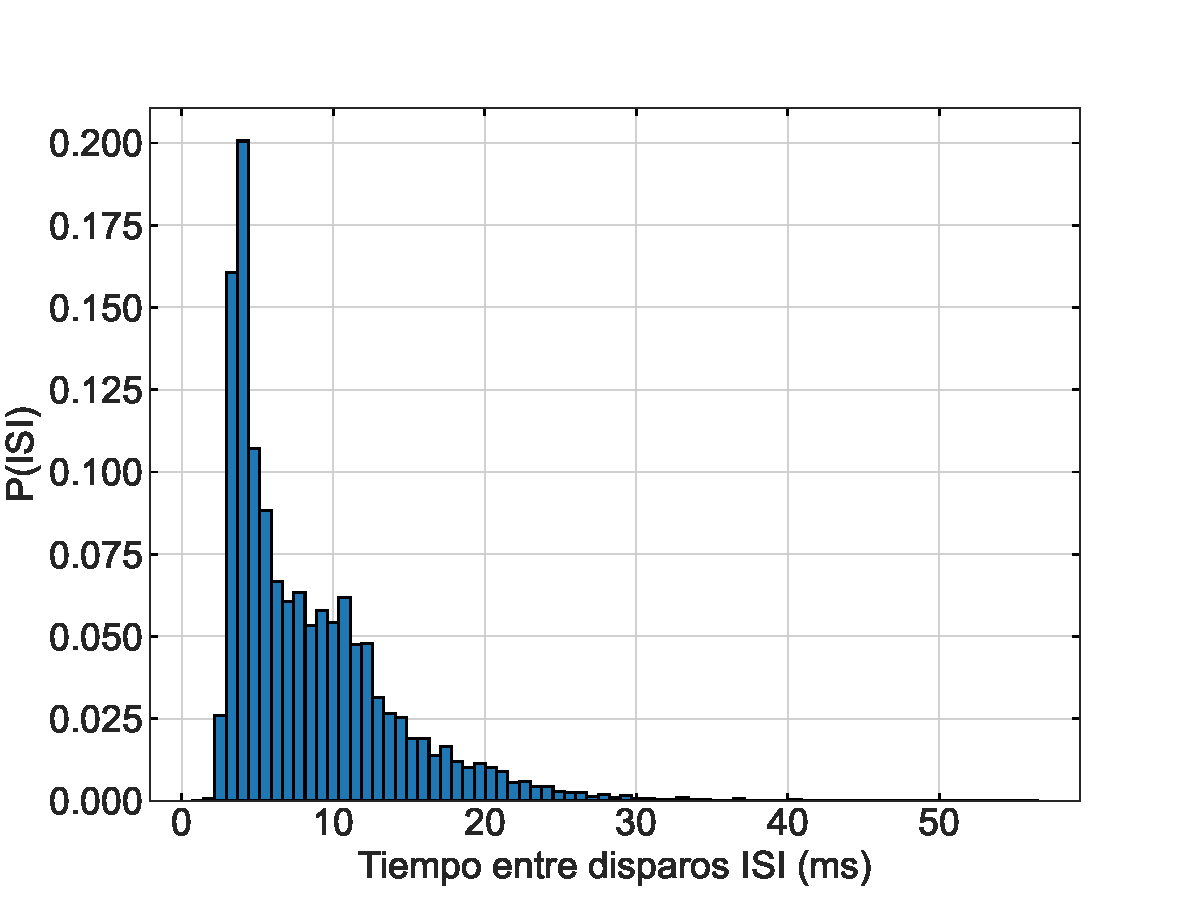
\includegraphics[width=\textwidth]{Figuras/histograma_ISI.pdf}
         \end{subfigure}
    \caption{Histograma de los intervalos de tiempo entre disparos (ISI).} 
    \label{fig:histISI}
\end{figure}
\newpage
Se calculó el valor medio de la distribución de valores de tiempo entre disparos $\langle \tau \rangle = 8.57$ ms y el desvío estándar $\sigma_\tau = 5.63$ ms. Se define el coeficiente de variabilidad CV como $CV = \frac{\sigma_\tau}{\langle \tau \rangle}$, en este caso se obtiene
\begin{equation}
    \text{CV} = 0.66.
\end{equation}
Se sabe que el valor de CV para un proceso de Poisson homogéneo es 1. En este caso, se obtiene un valor que difiere del mismo por lo que se puede concluir que la neurona no sigue un proceso de Poisson.


\section{Distribución del número de spikes}

\vspace{0.3cm}

Se realizó el histograma de la cantidad de spikes por realización, el resultado se muestra en la Fig. \ref{fig:histN}. Se calculó el valor medio de la cantidad de spikes por realización $\langle N \rangle = 117.01$ y el desvío estándar $\sigma_N = 13.53$.

Se define el factor de Fano $F$ como $F = \frac{\sigma_N^2}{\langle N \rangle}$, en este caso se obtiene
\begin{equation}
    F = 1.57.
\end{equation}

En un proceso de Poisson homogéneo el factor de Fano es 1. Como es de esperar por lo obtenido en la sección \ref{sec:ISI}, el factor de Fano difiere de 1 por lo que el experimento no coincide con un proceso de Poisson homogeneo. Además, en un proceso \textit{renewal} se cumple que $F = CV^2$. No obstante, no se verifica en este experimento ya que $CV^2 = 0.44 \neq F$.

\begin{figure}[ht]
    \centering
         \begin{subfigure}[b]{\linewidth}
            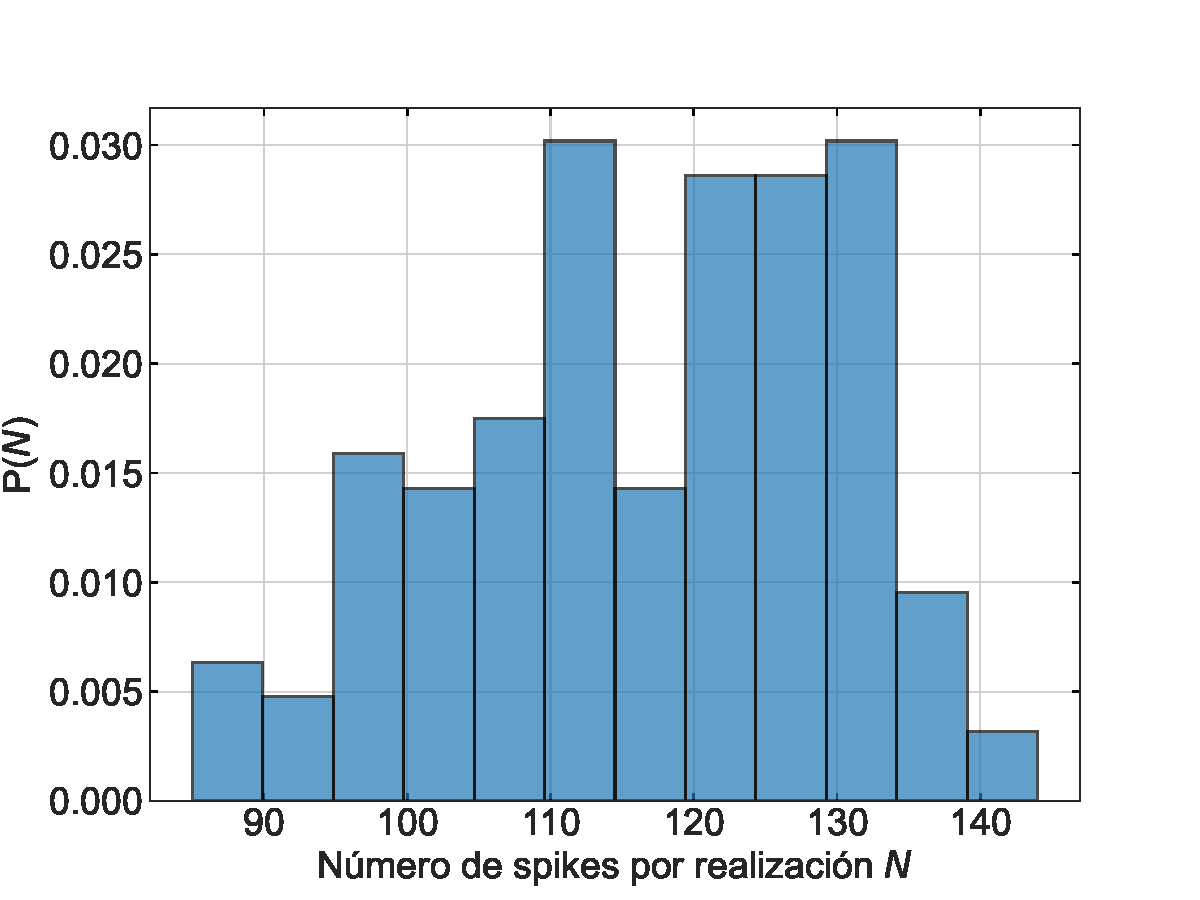
\includegraphics[width=\textwidth]{Figuras/histograma_spikes.pdf}
         \end{subfigure}
    \caption{Histograma del número de spikes $N$ por realización.} 
    \label{fig:histN}
\end{figure}

\section{Tasa de disparo en función del tiempo}

Se calculó la tasa de disparo o respuesta en función del tiempo $r(t)$. Para esto se tomaron ventanas de $20$ ms y se aplicó un suavizado por media móvil. Se realizó lo mismo para cada realización del experimento y se promedió la tasa de disparo, en cada ventana, para todas las realizaciones, obteniendo como resultado la tasa de disparo en función del tiempo. En la Fig. \ref{fig:tasadedisparo} se muestra el resultado obtenido.

\begin{figure}[ht]
    \centering
         \begin{subfigure}[b]{\linewidth}
            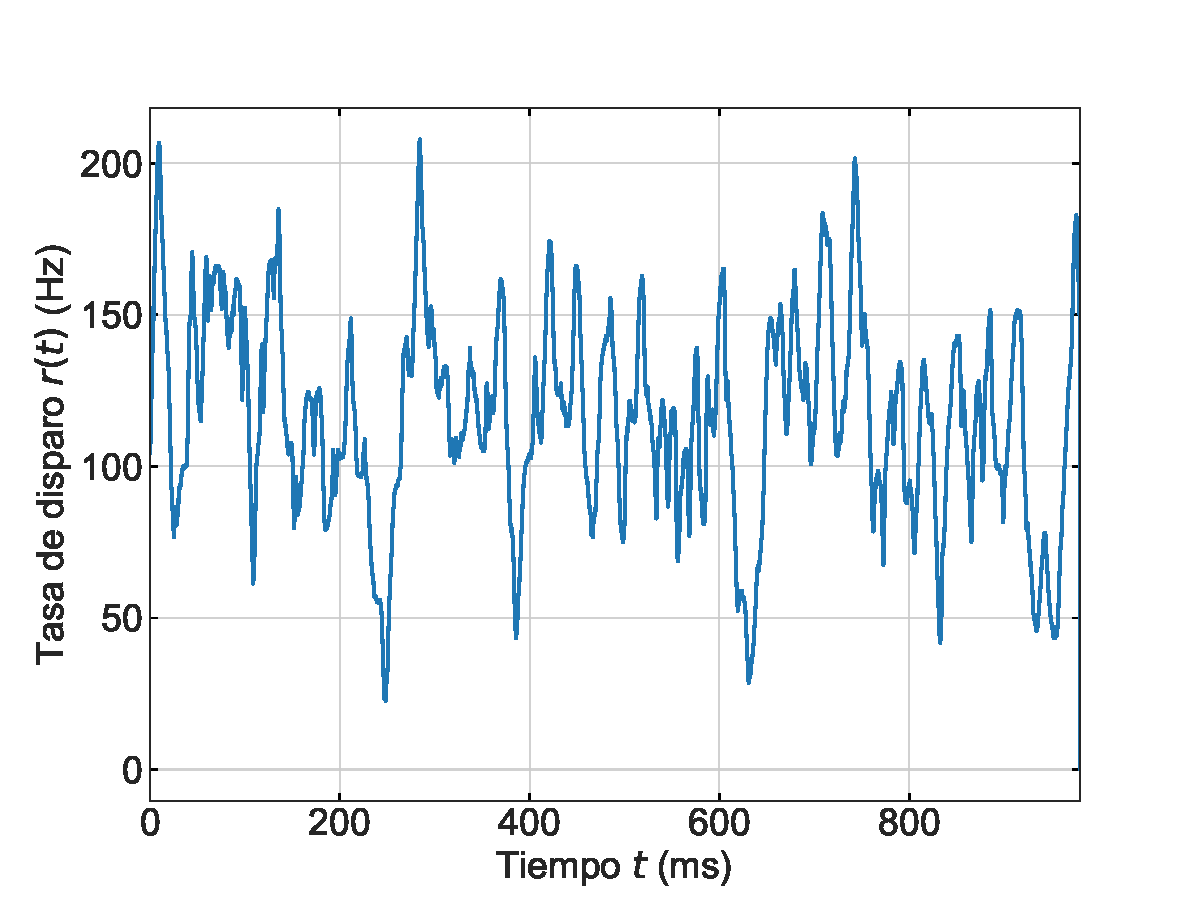
\includegraphics[width=\textwidth]{Figuras/tasa_disparo.pdf}
         \end{subfigure}
    \caption{Tasa de disparo en función del tiempo calculada en ventanas de $20$ ms utilizando un suavizado por media móvil.} 
    \label{fig:tasadedisparo}
\end{figure}

\section{Filtro asociado a la neurona}

\begin{figure*}[ht]
    \centering
            \begin{subfigure}[b]{\linewidth}
            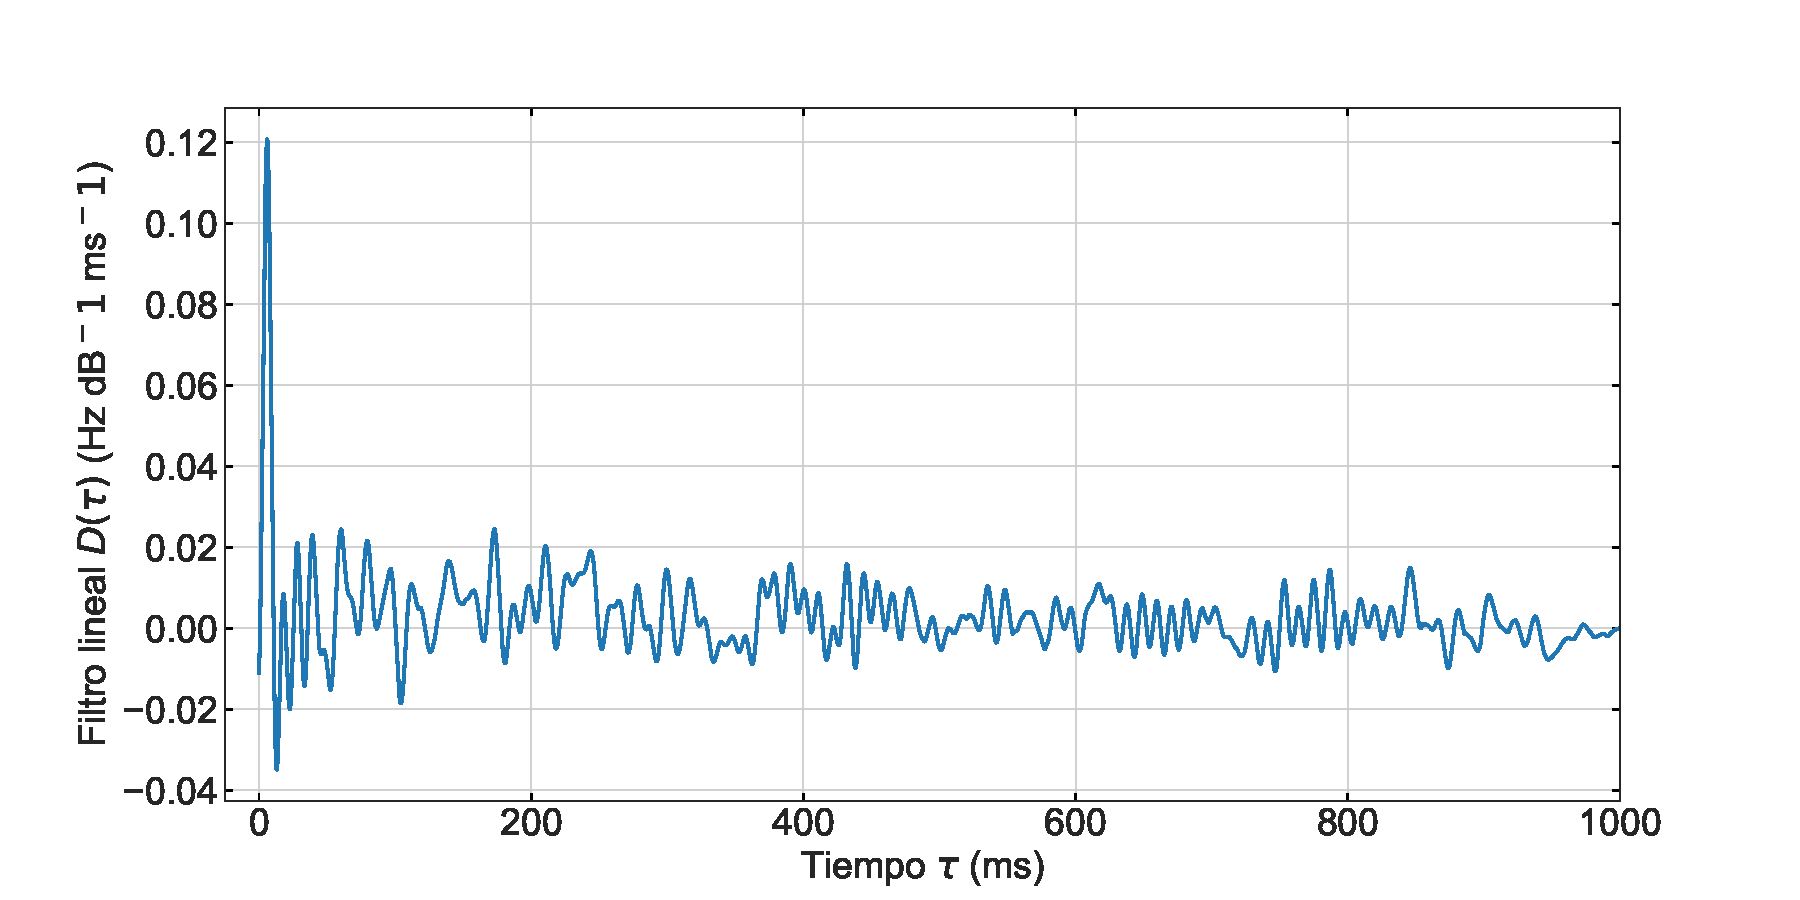
\includegraphics[width=\textwidth]{Figuras/filtro_lineal.pdf}
            \end{subfigure}
    \caption{Filtro lineal $D(\tau)$ que da la mejor la mejor predicción lineal de la respuesta dependiente del tiempo $r(t)$.} 
    \label{fig:filtrolineal}
\end{figure*}

Se calculó el filtro lineal asociado a la neurona $D(\tau)$ que da la mejor predicción lineal de la respuesta dependiente del tiempo $r(t)$. En la aproximación lineal, la respuesta se modela como una integral de solapamiento entre el filtro y el estímulo
\begin{equation}
r(t) = r_0 + \int_0^\infty \text{d}\tau ~ D(\tau) s (t-\tau).
\label{ec:solapamiento}
\end{equation}
Despreciando el tiempo de correlación del estímulo, es decir, considerando a dicho estímulo como ruido blanco gaussiano, se puede mostrar que el filtro lineal se calcula como 
\begin{equation}
    D(\tau) = \frac{1}{\sigma_s^2} ~ C(\tau),
\end{equation}
donde $\sigma_s$ es el desvío estándar del estímulo y $C(\tau)$ es el \textit{spike-triggered average} (STA). El STA se define como
\begin{equation}
    C(\tau) = \frac{1}{N}\sum_{\textit{spike}}^{N} s(t_{spike} - \tau),
\end{equation}
donde $t_{spike}$ es el tiempo que ocurre un spike y $N$ es la cantidad de spikes en una realización. Es decir, es el valor medio del estímulo en un tiempo $\tau$ antes que se dispare el spike. Se calculó $D(\tau)$ para cada realización y luego se promedió $D(\tau)$ entre todas las realizaciones. Este resultado se observa en la Fig. \ref{fig:filtrolineal}. Se obtuvo que el máximo valor de filtro está en aproximadamente $\tau \approx 5$ ms y a valores grandes de $\tau$ se observa que el filtro es ruidoso y oscila en un entorno de 0. 

Se puede ver de la curva obtenida que los valores de $\tau$ cercanos a $5$ ms son los que producen mayores valores de filtro y por lo tanto más aportan a la respuesta obtenida. De esta manera dichos valores de tiempo $\tau$ son los que más contribuyen a la integral de solapamiento (Ec. \ref{ec:solapamiento}) que modela la respuesta.

% Bibliography
%\renewcommand*{\bibfont}{\normalsize}
%\bibliography{Redes}

% Full bibliography added automatically for Optics Letters submissions; the following line will simply be ignored if submitting to other journals.
% Note that this extra page will not count against page length
%\bibliographyfullrefs{Redes}


\centerline{\rule{0.95\linewidth}{0.6pt}}

\clearpage 

\begin{onecolumn} % Activa una sola columna para el apéndice
\appendix
\section{Apéndice \label{codigo}}

\begin{lstlisting}[language=Python, caption={Implementación del método Runge-Kutta 4.}, label=python-code]

import numpy as np
import matplotlib.pyplot as plt
from scipy.stats import poisson
from scipy.optimize import curve_fit

#Ploteo 
import seaborn as sns
#sns.axes_style("whitegrid")
sns.set_style("ticks")

#Carga de datos
stimulus = np.loadtxt(r"../Redes-Neuronales/Practica_3/stimulus.dat")
tiempo = stimulus[:, 0]
estimulo = stimulus[:, 1]
spikes = np.loadtxt(r"../Redes-Neuronales/Practica_3/spikes.dat")
num_experimentos, num_pasos = spikes.shape

# Ploteo para la figura 1
fig1, ax1 = plt.subplots(figsize=(12,6))
ax1.plot(tiempo, estimulo, "-")
ax1.set_xlabel("Tiempo $t$ (ms)", fontsize=15)
ax1.set_ylabel("Estimulo (dB)", fontsize=15)
ax1.tick_params(direction='in', top=True, right=True, left=True, bottom=True)
ax1.tick_params(axis='x',rotation=0, labelsize=18, color='black')
ax1.tick_params(axis='y', labelsize=18, color='black')
ax1.set_xlim(0, 1000)
ax1.grid(True, linewidth=0.5, linestyle='-', alpha=0.9)
# Guardar figura 1
fig1.savefig(f"../Redes-Neuronales/Practica_3/resultados/estimulo_vs_t.pdf")
fig1.savefig(f"../Redes-Neuronales/Practica_3/resultados/estimulo_vs_t.png",
dpi=600)

x, y = np.meshgrid(np.arange(num_pasos)*0.1, np.arange(num_experimentos))
# Crear una mascara para valores iguales a 1
mascara = spikes == 1

# Ploteo para la figura 2
fig2, ax2 = plt.subplots(figsize=(12,6)) 
ax2.scatter(x[mascara], y[mascara], marker='|', s=50)
ax2.set_xlabel("Tiempo $t$ (ms)", fontsize=15)
ax2.set_ylabel("Realizacion", fontsize=15)
ax2.tick_params(direction='in', top=True, right=True, left=True, bottom=True)
ax2.tick_params(axis='x',rotation=0, labelsize=18, color='black')
ax2.tick_params(axis='y', labelsize=18, color='black')
ax2.set_xlim(0, 1000)
ax2.set_ylim(0, num_experimentos)
ax2.grid(True, linewidth=0.5, linestyle='-', alpha=0.9)
# Guardar figura 2
fig2.savefig(f"../Redes-Neuronales/Practica_3/resultados/reailzaciones_vs_t.pdf")
fig2.savefig(f"../Redes-Neuronales/Practica_3/resultados/realizaciones_vs_t.
png", dpi=600)

#Ejercicio 1

diffs = []

for i in range(num_experimentos):
    diff = np.diff(np.where(spikes[i, :] == 1)[0]) * 0.1
    diffs.extend(diff)

# Ploteo para la figura 3
fig3, ax3 = plt.subplots(figsize=(8,6)) 
ax3.hist(diffs, bins=75, density=True, edgecolor='black')
ax3.set_xlabel("ISI (ms)", fontsize=15)
ax3.set_ylabel(r"P(ISI)", fontsize=15)
ax3.tick_params(direction='in', top=True, right=True, left=True, bottom=True)
ax3.tick_params(axis='x',rotation=0, labelsize=18, color='black')
ax3.tick_params(axis='y', labelsize=18, color='black')
ax3.grid(True, linewidth=0.5, linestyle='-', alpha=0.9, zorder=0)
ax3.set_zorder(1)
# Guardar figura 3
fig3.savefig(f"../Redes-Neuronales/Practica_3/resultados/histograma_ISI.pdf")
fig3.savefig(f"../Redes-Neuronales/Practica_3/resultados/histograma_ISI.png",
dpi=600)

mean = np.mean(diffs)
print(f'Promedio: {mean:.2f} ms')
std_deviation = np.std(diffs)
print(f'Desviacion estandar: {std_deviation:.2f} ms')
CV = std_deviation/mean 
print(f'CV: {CV:.2f}')

#Ejercicio 2

spikes_exp = np.zeros(num_experimentos)
for i in range(num_experimentos):
    spikes_exp[i] = np.sum(spikes[i, :] == 1)

fig4, ax4 = plt.subplots(figsize=(8,6)) 
ax4.hist(spikes_exp, bins=12, density=True, edgecolor='black', alpha=0.7)
ax4.set_xlabel("Numero de spikes por realizacion $N$", fontsize=15)
ax4.set_ylabel(r"P($N$)", fontsize=15)
ax4.tick_params(direction='in', top=True, right=True, left=True, bottom=True)
ax4.tick_params(axis='x',rotation=0, labelsize=18, color='black')
ax4.tick_params(axis='y', labelsize=18, color='black')
ax4.grid(True, linewidth=0.5, linestyle='-', alpha=0.9, zorder = 0)
ax4.set_zorder(1)
# Guardar figura 4
fig4.savefig(f"../Redes-Neuronales/Practica_3/resultados/histograma_spikes.pdf")
fig4.savefig(f"../Redes-Neuronales/Practica_3/resultados/histograma_spikes.png",
dpi=600)

# Calcular el promedio y la desviacion estandar de la cantidad de spikes 
por experimento
promedio_spikes = np.mean(spikes_exp)
desviacion_estandar_spikes = np.std(spikes_exp)
print(f'Promedio de spikes por experimento: {promedio_spikes:.2f}')
print(f'Desviacion Estandar de spikes por experimento:
{desviacion_estandar_spikes:.2f}')
F = (desviacion_estandar_spikes**2)/promedio_spikes
print(f'Factor de Fano: {F:.2f}')

#Ejercicio 3
w = 200
tasa_de_disparo = np.zeros(len(tiempo))

for t in range(len(tiempo)-w):
    inicio = t  
    fin = inicio + w
    tasas_de_disparo_en_ventana = np.zeros(num_experimentos)

    for i in range(num_experimentos):
        tasas_de_disparo_en_ventana[i] = (np.sum(spikes[i, inicio:fin] == 1)/w)
        *10000
    
    tasa_de_disparo[t] = np.mean(tasas_de_disparo_en_ventana)
            
# Ploteo para la figura 5
fig5, ax5 = plt.subplots(figsize=(8,6)) 
ax5.plot(tiempo, tasa_de_disparo, "-")
ax5.set_xlabel(r"Tiempo $t$ (ms)", fontsize=15)
ax5.set_ylabel(r"Tasa de disparo $r(t)$ (Hz)", fontsize=15)
ax5.tick_params(direction='in', top=True, right=True, left=True, bottom=True)
ax5.tick_params(axis='x',rotation=0, labelsize=18, color='black')
ax5.tick_params(axis='y', labelsize=18, color='black')
ax5.set_xlim(0, 980)
ax5.grid(True, linewidth=0.5, linestyle='-', alpha=0.9)
# Guardar figura 5
fig5.savefig(f"../Redes-Neuronales/Practica_3/resultados/tasa_disparo.pdf")
fig5.savefig(f"../Redes-Neuronales/Practica_3/resultados/tasa_disparo.png",
dpi=600)

# Ploteo para la figura 6
fig6, ax6 = plt.subplots(figsize=(8,6)) 
ax6.hist(tasa_de_disparo, bins=30, density=True, edgecolor='black', alpha=0.7)
ax6.set_xlabel("Tasa de disparo", fontsize=15)
ax6.set_ylabel(r"P($r$)", fontsize=15)
ax6.tick_params(direction='in', top=True, right=True, left=True, bottom=True)
ax6.tick_params(axis='x',rotation=0, labelsize=18, color='black')
ax6.tick_params(axis='y', labelsize=18, color='black')
ax6.grid(True, linewidth=0.5, linestyle='-', alpha=0.9, zorder = 0)
ax6.set_zorder(1)
# Guardar figura 6
fig6.savefig(f"../Redes-Neuronales/Practica_3/resultados/histograma_tasa_disparo.
pdf")
fig6.savefig(f"../Redes-Neuronales/Practica_3/resultados/histograma_tasa_disparo
.png",dpi=600)

tau_range = np.arange(0, 10002, 1) 
C = np.zeros(len(tau_range))   

for i in range(num_experimentos):
    #print(i)
    spikes_indices = np.where(spikes[i, :] == 1)[0]
    for tau in tau_range:
        C_exp = 0
        for spike_index in spikes_indices:
            t_i = spike_index
            if t_i > tau:
                s = stimulus[t_i - tau][1]
                C_exp += s
        C[tau] += C_exp/(len(spikes_indices))

var = np.var(estimulo)

C = C/num_experimentos
D = C/var

# Ploteo para la figura 7
fig7, ax7 = plt.subplots(figsize=(12,6)) 
ax7.plot(tau_range*0.1, D, "-")
ax7.set_xlabel(r"$\tau$ (ms)", fontsize=15)
ax7.set_ylabel(r"Filtro lineal $D(\tau)$ (Hz dB$^-1$ ms$^-1$)", fontsize=15)
ax7.tick_params(direction='in', top=True, right=True, left=True, bottom=True)
ax7.tick_params(axis='x',rotation=0, labelsize=18, color='black')
ax7.tick_params(axis='y', labelsize=18, color='black')
ax7.set_xlim(-25, 1000)
ax7.grid(True, linewidth=0.5, linestyle='-', alpha=0.9)
# Ploteo para la figura 7
fig7.savefig(f"../Redes-Neuronales/Practica_3/resultados/filtro_lineal.pdf")
fig7.savefig(f"../Redes-Neuronales/Practica_3/resultados/filtro_lineal.png", 
dpi=600)

\end{lstlisting}
\end{onecolumn}

\end{document}


